% File              : manual.tex
% Author            : Marcos Horro <marcos.horro@udc.gal>
% Date              : Mar 24 Dec 2019 19:31:10 MST
% Last Modified Date: Mér 25 Dec 2019 18:35:55 MST
% Last Modified By  : Marcos Horro <marcos.horro@udc.gal>
\documentclass[a4paper,12pt]{memoir}
% For TeXstudio users:
% !TeX spellcheck = en_US

\usepackage[ruled,vlined]{algorithm2e}
\usepackage{graphicx}
\usepackage{amsthm}
\usepackage{tikz}
\usetikzlibrary{arrows}

%\theoremstyle{definition}
\newtheorem{definition}{Definition}[]
\newtheorem{corollary}{Corollary}[]




% Title Page
\title{\textbf{MACVETH}: \textbf{M}ulti-dimensional \textbf{A}rray
    \textbf{C}-compiler for \textbf{VE}ctorizing
    \textbf{T}ensors for \textbf{H}PC applications}
\author{Marcos Horro}
\date{}

%%%%%%%%%%%%%%%%%%%%%%%%%%%%%%%%%%%%%
\begin{document}

\maketitle

%%%%%%%%%%%%%%%%%%%%%%%%%%%%%%%%%%%%%
\begin{abstract}
	This document presents the Multi-dimensional Array C-compiler for VEctorization
	and Transformation in HPC applications (MACVETH) compiler tool. Details
	regarding implementation and design decision are explained in detail. For
	specific implementation details refer to the proper source code, which is also
	documented using Doxygen.
\end{abstract}

\chapter{MACVETH}
\label{chapter:Intro}
% PACT ABSTRACT
%Modern optimizing compilers implement robust auto-vectorization techniques 
%targeting rich SIMD ISAs. However the typical practice is to generate 
%machine-specific assembly code, which exploits the SIMD units of the targeted 
%processor.  In this work we take a different approach, by developing a 
%source-to-source compilation framework targeting the automatic vectorization 
%of 
%specific loop regions. We implement vectorization using an intrinsics-style 
%approach, to facilitate portability to a variety of concrete SIMD ISAs. We 
%develop machine-independent cost-driven algorithms to pack efficiently 
%arbitrary operands and operations into SIMD vectors. Specifically, we support 
%vector packing across multiple distinct loop nests to maximize vector 
%occupancy 
%in particular when loops have a very small trip count. Experimental results 
%are 
%presented for a large set of vectorizable loop shapes, and for several key 
%deep 
%learning inference programs, demonstrating the benefits of random vector 
%packing for efficient and portable vectorization of highly rectangular loops.



%Despite of the extraordinary performance with regard to the optimizations that
%compilers, e.g. ICC, Clang/LLVM, GNU/GCC, may be able to do all over programs, 
%they 
%also
%show limitations when it comes to vectorization. There are cases where either
%they may not vectorize the code at all or even deliver worse performance than a
%sequential version of it. This is a common scenario when the region of interest
%in the code to vectorize is not regular. We may define the regularity of a code
%as the presence of patterns whose accesses to the elements (e.g.
%multi-dimensional arrays) are performed in a sequential and contiguous manner,
%e.g. map operations. On the other hand, reductions are a type of operations
%that, by nature,
%do not fully exploit the capacity of vector operands. Current data placement or
%packing techniques are meant just for loading and storing data from or to
%memory, without performing any other logic than that. Potential improvements
%regarding the vector occupancy by complex and smart packing techniques may lead
%to major gains in performance. Picture the following example: within the same
%loop we have two different and contiguous reductions. This is a common pattern
%that can be found after the fusion of different loops, for instance, in codes
%that perform convolutions. Assuming a vector size of four elements, a smart way
%of computing this code is by



Modern optimizing compilers implement robust auto-vectorization techniques 
targeting rich SIMD ISAs. A typical approach is to generate machine-specific 
assembly, exploiting SIMD units of a target processor. By default, most of the 
techniques employed by auto-vectorizers are conservative, and will only apply 
if certain patterns are found in the program~\cite{citeneeded}. Vectorization 
also relays in the computation of a cost model. Each compiler has its own 
algorithm to compute this value in charge to decide whether the vectorization 
is placed or not for a certain region of code. For instance, GCC/GNU and 
Clang/LLVM use both Loop Level Vectorizer (LLV) and Superword Level Parallelism 
(SLP), the first one just in one pass and the last one in two passes, but both 
use a similar approach in order to asses whether the vectorization is 
profitable or not: unroll loops using different vector factors, compute de cost 
of each vector instruction and compare total cost to the scalar or not 
vectorized cost.

% Different ISA
In an orthogonal dimension, the quality of SIMD code is affected by the 
knowledge of the architecture where it is being compiled. Nevertheless, some 
information regarding the SIMD instructions performance may be missing or 
non-disclosed by the manufacturer. This information can be used to determine 
whether a vector operation is detrimental or not, i.e. for building a cost 
model. There may be architectures using the same ISA and, therefore, where the 
vectorization can be done using exactly the same instructions, but because of 
their architectural features, performance might be completely different, 
leading to the synthesis of particular solutions on each case. Thus, the only 
manner of 
disclosing these features is by reverse-engineering each architecture. This 
process is 
tedious and complex since there are many different instructions (CISC 
architectures) whose 
performance may also vary depending on the packing of data they use. 
Nevertheless, uops.info~\cite{bib:uops} provides performance information of 
many 
assembly instructions in all different variants (order and type of operands, 
i.e. register, memory, immediate values, masks, etc.) for various 
architectures. This information can be used by compilers to improve their 
accuracy when computing its vectorization cost model. Nonetheless, this 
information is 
restricted only 
to 
assembly instructions, not those ``high-level'' SIMD intrinsics such as Intel's 
(SSE, AVX) or ARM's (NEON, SVE). Main reason is that not all SIMD macros or 
idioms have a 1:1 translation onto assembly, but some of them might generate a 
set of instructions and/or data movements.


\begin{figure*}
	\centering
	\includegraphics[width=.7\textwidth]{img/MACVETH.pdf}
	\caption{High-level picture of the MACVETH pipeline compiler, based on the 
		Clang/LLVM Tool Framework.}
	\label{fig:MACVETHarch}
\end{figure*}

Hence, in this work we take a different approach than ``traditional'' 
auto-vectorizers, by developing MACVETH, which 
stands 
for Multi-dimensional Array C-compiler for
VEctorizating Tensors for HPC applications. This is a 
source-to-source compilation framework targeting the automatic vectorization 
of 
specific loop and non-loop regions. We implement vectorization using an 
SIMD-intrinsics ´style 
approach, to facilitate portability to a variety of concrete SIMD ISAs. We 
develop machine-independent cost-driven algorithms to pack efficiently 
arbitrary operands and operations into SIMD vectors. Specifically, we support 
vector packing across multiple distinct loop nests to maximize vector 
occupancy 
in particular when loops have a very small trip count. Experimental results 
are 
presented for a large set of vectorizable loop shapes, and for several key 
deep 
learning inference programs, demonstrating the benefits of random vector 
packing for efficient and portable vectorization of highly rectangular loops.


\newpage
\chapter{Intermediate Representations (IR)}
\label{chapter:IR}



MACVETH compiler handles different abstraction levels or intermediate
representations in order to facilitate the vectorization process. As MACVETH is 
based in Clang/LLVM~\cite{bib:clang}, the first abstraction layer lays on the 
Clang AST. This representation allows to identify the regions of interest for 
the translation, to extract 

\section{MACVETH Expressions: MVExpr}
Clang implements complex expressions in order to handle any form or type of
code. They
provide many possibilities
when it comes to parse exactly the code. Nonetheless, in our case we are
interested in a small set of operations, so we created basically a wrap for this
purpose. MVExpr is an abstract class that can be specialized for any type we
want to represent from the Clang AST. Besides, the idea of this class is to
provide a set of non-standard transformations for the expressions, e.g.
unrolling. Thus, MVExpr are instantiated using a factory.

We have implemented the following specializations, which are enough in order to
represent any value reference:

\begin{itemize}
	\item \textbf{MVExprArray}: represents any N-dimensional expression in the
	      code. It
	      holds information of the number of dimensions and name or value of the
	      indices. This class is very useful when performing unrolling, as it 
	      provides methods for computing deltas between two indices of the same 
	      or different form, e.g. $(i+1)*2$ vs. $(i+1)*4$.
	\item \textbf{MVExprVar}: regardless the type of the variable, this
	      abstraction
	      represents, basically, any \texttt{DeclRefExpr} from the Clang AST.
	\item \textbf{MVExprLiteral}: any integer, float, double, char, etc. value.
	\item \textbf{MVExprFunc}: this is a recursive abstraction which holds the
	      name of the function and the parameters it receives. Parameters are 
	      also MVExpr type.
\end{itemize}

\section{Three-Address Code IR: TAC}
Statements may differ in number of operations, data handled, or even types. 
This makes difficult to handle them properly.  The Three-Address Code (TAC) 
representation is used to translate any statement ($S$) into a
set of Single Stament Assignment (SSA), which have the same length. There are 
different ways of representing this format, but in our case we use quadruples, 
as described in Definition~\ref{def:TAC}.

\theoremstyle{definition}
\begin{definition}\label{def:TAC}
	A three-address code or TAC is a 4-tuple TAC=(a,b,c,$\oplus$) which 
	represents the 	assignment of the $b \oplus c$ operation as $a=b \oplus c$. 
	If the $\oplus$ operator is unary, then $c$ is null, so $a=\oplus b$.
\end{definition}

Thus, any statement of a program is composed by a concatenation of operations, 
e.g. assignment ($=$, $+$, a function, etc.), 
which are 
split onto TACs respecting  their operational order. Thus, when any statement 
generates more than one TAC, temporal registers are generated, in a 
SSA-fashion. Those assignments are 
responsible for connecting TACs and, therefore, represent the logical order of 
the original statement. In essence, those TAC connections generate a tree 
structure. In order to 
perform this translation, we have 
implemented a recursive process which is listed in 
Algorithm~\ref{alg:stmtToTAC}. 

\begin{algorithm}[h]\label{alg:stmtToTAC}
	\SetAlgoLined
	\KwIn{Stmt S}
	\KwResult{Set of TAC}
	L $\leftarrow$ \{\}\;
	Res $\leftarrow$ getResultOrTempReg(S)\;
	Lhs $\leftarrow$ getLHS(S)\;
	Rhs $\leftarrow$ getRHS(S)\;
	\If{isNonTerminal(Lhs)}{
		TAC $\leftarrow$ translateStmtToTAC(Lhs)\;
		addTacToList(L, TAC)\;
		Lhs $\leftarrow$ TAC.Res\;
	}
	\If{isNonTerminal(Rhs)}{
		TAC $\leftarrow$ translateStmtToTAC(Rhs)\;
		addTacToList(L, TAC)\;
		Rhs $\leftarrow$ TAC.Res\;
	}
	addTacToList(L, \{Res, Lhs, Rhs, getOp(S)\})\;
	return L\;
	\caption{translateStmtToTAC}
\end{algorithm}

\begin{corollary}\label{cor:TAC}
	Any statement $S$ can be represented as a set of interconnected TACs:
	$S = \{TAC\}$
\end{corollary}

This representation is widely used in compilers. The main advantages of it
resides in the simplicity of handling operations with the same number of
operands. Besides, this format is very easy to handle in programmatically terms.


Unrolling is also performed using this format, following the iterative process
listed in
Algorithm~\ref{alg:TACunrolling}.

\begin{algorithm}[H]\label{alg:TACunrolling}
	\SetAlgoLined
	\KwIn{TAC list $T$, Unrolling Factor $UF$, Loop nests $LN$}
	\KwResult{TAC list $T'$}
	$T'$ = \{\}\;
	\ForEach{LN} {
		\For{step = 0; step++ $<$ UF;} {
			\ForEach{TAC in T} {
				NewTac = \{\}\;
				\ForEach{Expr in TAC} {
					NewExpr $\leftarrow$ unrollExpr(step, LN, Expr)\;
					NewTac $\leftarrow$ placeExprInTac(NewExpr)\;
				}
				$T'$ $\leftarrow$ add(NewTac)\;
			}
		}
	}
	return $T'$\;
	\caption{Unrolling TAC list}
\end{algorithm}


\section{Computation Directed Acyclic Graph (CDAG)}
When it comes to schedule the different TACs in the ROI of our program, we need
a representation which can handle the dependencies between the statements and
some structures that store the information about the placement of them in the
execution. For this purpose we use a Computation Directed Acyclic Graph or
CDAG~\cite{bib:CDAGdefinition}. Informally, it is a forest that represents the
TACs as a set of nodes, where
each node can be a memory operation (load, store) or any other type of
operation (addition, multiplication, built-in function, etc.). Connections
between those nodes represent data dependencies. Formal
definition of the CDAG we have implemented can be found in
Definition~\ref{def:CDAG}. It is, essentially, a slight variation
of the definition given in~\cite{bib:CDAGdefinition}.

\theoremstyle{definition}
\begin{definition}\label{def:CDAG}
	A computation directed acyclic graph (CDAG) is a 4-tuple C=(I,V,E,O) of
	finite sets such that: (1) $I \subseteq V, O \subseteq (V-I)$; (2) $E
		\subseteq V
		\times V$ is the set of arcs; (3) $G=(V,E) \subseteq C$ is a subgraph 
		of C
\end{definition}

The importance of this structure is, in essence, to detect data races and to 
perform any kind of variation in the placement of operations, if possible. 
Nonetheless, this topic is not to be discussed in this work, since MACVETH uses 
the CDAG for sorting nodes in a topological order and detect patterns such as 
reductions.

\begin{figure}[h]
	\centering
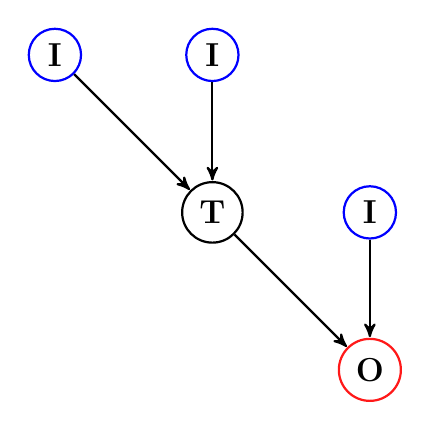
\begin{tikzpicture}[
	->,
	>=stealth',
	shorten >=.2pt,
	auto,
	node distance=2cm,
	thick,
	tmp node/.style={circle,draw,font=\large\bfseries},
	in node/.style={circle,draw=blue!100,font=\large\bfseries},
	out node/.style={circle,draw=red!90,font=\large\bfseries}
]

\node[in node] (1) {I};
\node[in node] (2) [right of=1] {I};
\node[tmp node] (3) [below of=2] {T};
\node[in node] (4) [right of=3] {I};
\node[out node] (5) [below of=4] {O};
%\node[main node] (1) {In};
%\node[main node] (2) [below left of=1] {2};
%\node[main node] (3) [below right of=2] {3};
%\node[main node] (4) [below right of=1] {4};

\path[every node/.style={font=\sffamily\small}]
(1) edge node [left] {} (3)
(2) edge node [left] {} (3)
(3) edge node [left] {} (5)
(4) edge node [left] {} (5)
;
%(1) edge node [left] {0.6} (4)
%%edge [bend right] node[left] {0.3} (2)
%edge [loop above] node {0.1} (1)
%(2) edge node [right] {0.4} (1)
%edge node {0.3} (4)
%edge [loop left] node {0.4} (2)
%edge [bend right] node[left] {0.1} (3)
%(3) edge node [right] {0.8} (2)
%edge [bend right] node[right] {0.2} (4)
%(4) edge node [left] {0.2} (3)
%edge [loop right] node {0.6} (4)
%edge [bend right] node[right] {0.2} (1);
\end{tikzpicture}
\caption{Graphical example of CDAG}
\label{fig:GraphCDAG}
\end{figure}

Figure~\ref{fig:GraphCDAG} shows the graphical representation of a CDAG 
generated from the code. Key idea of this IR is to provide information 
regardin

\section{VectorIR}
In order to approach the different architectures when generating instructions,
we need a generic vector representation of the vector instructions we want to
have in our program. For this purpose, MACVETH uses the VectorIR, that basically
wraps a set of nodes from the CDAG onto a common structure which represent a 
vector operation. This vector representation is linked to the target 
architecture and ISA, as the maximum number of elements in a vector operation 
depends on the type of data and the maximum vector width in the architecture. 
Thus, each vector operation will also depend of two vector operands, which are, 
as well, a wrap of set of memory or result nodes in the CDAG. 
Definition~\ref{def:VectorIR} synthesis in a more formal manner this paragraph.

\theoremstyle{definition}
\begin{definition}\label{def:VectorIR}
	A vector operation is a 4-tuple $VIR=(\oplus, VOp_{R}, VOp_{1}, 
	VOp_{2})$ such that: (1) $|VOp_{i}| \leq ISA_{width}$, (2) $VOp_{i} 
	\subseteq C$, (3) $\forall i,j / VOp_{i} \cap VOp_{j} = \emptyset$
\end{definition}

To wrap up: VectorIR is a generic way of representing vector operations for the 
different
architectures. Because of this, at this stage there is no fusing operations or
any other kind of target-specific optimizations. The concrete backend will be in
charge of doing this. For instance, AVX introduced the fuse add-multiplication
instructions often called FMAs, which as their name suggest fuse additions and
multiplication onto a single operation; however they are only available for FP
operations and, therefore, not for integers. It would be pointless to tackle
all these issues in this representation that is why this is done in the AVX
backend instead.




\newpage
\chapter{Software Architecture}
MACVETH is built using LLVM framework in order to take advantage of the
sophisticated AST created when parsing files.

\newpage
\bibliographystyle{unsrt}
\bibliography{sample}

\end{document}
%%%%%%%%%%%%%%%%%%%%%%%%%%%%%%%%%%%%%
